\documentclass{article}
\usepackage[utf8]{inputenc}
\usepackage{tikz}

\title{RegAut afl. 3}
\author{Anders Kostending, 201303537}
\date{May 2014}

\begin{document}

\maketitle

\section*{Kommentarer}
    Jeg brugte første $\Lambda$-eliminering til at fjerne alle lambda-transitionerne den givne i NFA. Derefter lavede jeg en transitions-tabel, som jeg brugte til at lave detaminiseringen fra NFA til min FA. 
    

\section*{NFA$^*$}
    

\begin{center}
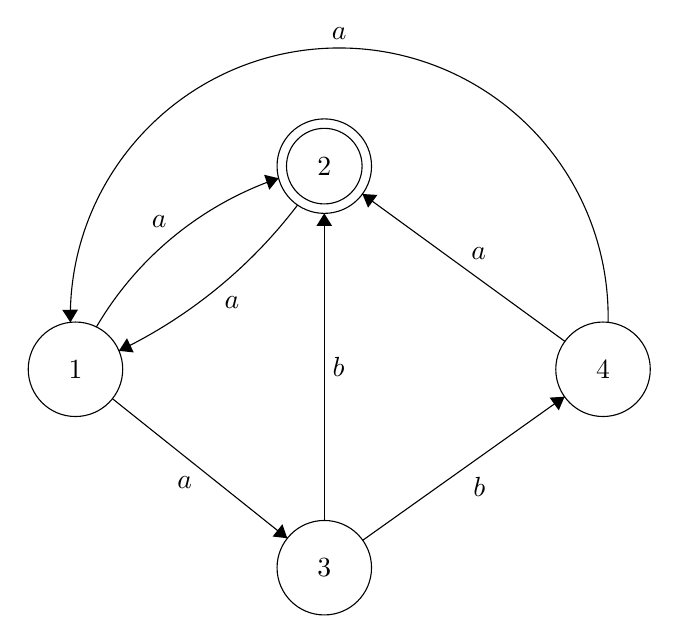
\begin{tikzpicture}[scale=0.2]
\tikzstyle{every node}+=[inner sep=0pt]
\draw [black] (15.8,-28.3) circle (3);
\draw (15.8,-28.3) node {$1$};
\draw [black] (31.6,-15.4) circle (3);
\draw (31.6,-15.4) node {$2$};
\draw [black] (31.6,-15.4) circle (2.4);
\draw [black] (31.6,-40.9) circle (3);
\draw (31.6,-40.9) node {$3$};
\draw [black] (49.3,-28.3) circle (3);
\draw (49.3,-28.3) node {$4$};
\draw [black] (17.13,-25.613) arc (149.65424:108.80599:21.405);
\fill [black] (28.7,-16.17) -- (27.78,-15.95) -- (28.11,-16.9);
\draw (21.11,-19.35) node [above] {$a$};
\draw [black] (29.902,-17.872) arc (-37.24115:-64.29862:31.291);
\fill [black] (18.56,-27.13) -- (19.5,-27.23) -- (19.07,-26.33);
\draw (25.74,-23.67) node [below] {$a$};
\draw [black] (18.15,-30.17) -- (29.25,-39.03);
\fill [black] (29.25,-39.03) -- (28.94,-38.14) -- (28.32,-38.92);
\draw (22.74,-35.09) node [below] {$a$};
\draw [black] (31.6,-37.9) -- (31.6,-18.4);
\fill [black] (31.6,-18.4) -- (31.1,-19.2) -- (32.1,-19.2);
\draw (32.1,-28.15) node [right] {$b$};
\draw [black] (34.04,-39.16) -- (46.86,-30.04);
\fill [black] (46.86,-30.04) -- (45.91,-30.1) -- (46.49,-30.91);
\draw (41.45,-35.1) node [below] {$b$};
\draw [black] (46.88,-26.53) -- (34.02,-17.17);
\fill [black] (34.02,-17.17) -- (34.38,-18.04) -- (34.97,-17.23);
\draw (41.4,-21.35) node [above] {$a$};
\draw [black] (15.476,-25.321) arc (181.16716:-1.16716:17.077);
\fill [black] (15.48,-25.32) -- (15.96,-24.51) -- (14.96,-24.53);
\draw (32.55,-7.4) node [above] {$a$};
\end{tikzpicture}
\end{center}

    \begin{table}
        \centering
        \begin{tabular}{l|lll|ll}
        \hline
        q & $\delta(q,a)$   & $\delta(q,b)$ & $\delta(q,\Lambda)$ & $\delta^*(q,a)$     & $\delta^*(q,b)$   \\
        \hline
        1 & 2,3 & Ø & Ø      & 2,3   & Ø   \\
        2 & 1   & Ø & Ø      & 1     & Ø   \\
        3 & Ø   & 4 & Ø      & Ø     & 2,4 \\
        4 & 4   & Ø & 2      & 1,2,3 & Ø   \\
        \end{tabular}
    \end{table}
    
\section*{FA}
    \begin{center}
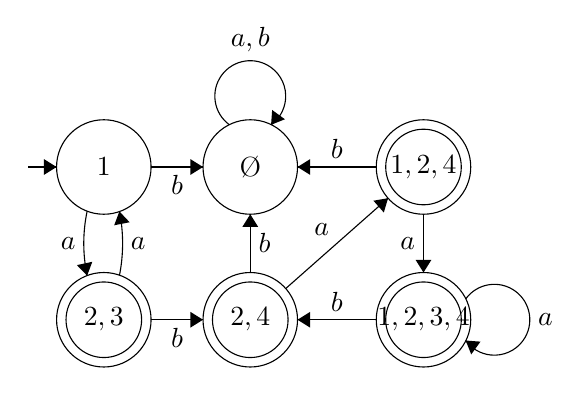
\begin{tikzpicture}[scale=0.2]
\tikzstyle{every node}+=[inner sep=0pt]
\draw [black] (9.2,-10.4) circle (3);
\draw (9.2,-10.4) node {$1$};
\draw [black] (9.2,-20.1) circle (3);
\draw (9.2,-20.1) node {$2,3$};
\draw [black] (9.2,-20.1) circle (2.4);
\draw [black] (18.5,-20.1) circle (3);
\draw (18.5,-20.1) node {$2,4$};
\draw [black] (18.5,-20.1) circle (2.4);
\draw [black] (29.5,-10.4) circle (3);
\draw (29.5,-10.4) node {$1,2,4$};
\draw [black] (29.5,-10.4) circle (2.4);
\draw [black] (29.5,-20.1) circle (3);
\draw (29.5,-20.1) node {$1,2,3,4$};
\draw [black] (29.5,-20.1) circle (2.4);
\draw [black] (18.5,-10.4) circle (3);
\draw (18.5,-10.4) node {$Ø$};
\draw [black] (4.4,-10.4) -- (6.2,-10.4);
\fill [black] (6.2,-10.4) -- (5.4,-9.9) -- (5.4,-10.9);
\draw [black] (12.2,-10.4) -- (15.5,-10.4);
\fill [black] (15.5,-10.4) -- (14.7,-9.9) -- (14.7,-10.9);
\draw (13.85,-10.9) node [below] {$b$};
\draw [black] (8.143,-17.305) arc (-167.99104:-192.00896:9.875);
\fill [black] (8.14,-17.3) -- (8.47,-16.42) -- (7.49,-16.63);
\draw (7.43,-15.25) node [left] {$a$};
\draw [black] (10.194,-13.22) arc (11.19636:-11.19636:10.456);
\fill [black] (10.19,-13.22) -- (9.86,-14.1) -- (10.84,-13.91);
\draw (10.89,-15.25) node [right] {$a$};
\draw [black] (12.2,-20.1) -- (15.5,-20.1);
\fill [black] (15.5,-20.1) -- (14.7,-19.6) -- (14.7,-20.6);
\draw (13.85,-20.6) node [below] {$b$};
\draw [black] (20.75,-18.12) -- (27.25,-12.38);
\fill [black] (27.25,-12.38) -- (26.32,-12.54) -- (26.98,-13.29);
\draw (23.04,-14.76) node [above] {$a$};
\draw [black] (18.5,-17.1) -- (18.5,-13.4);
\fill [black] (18.5,-13.4) -- (18,-14.2) -- (19,-14.2);
\draw (19,-15.25) node [right] {$b$};
\draw [black] (29.5,-13.4) -- (29.5,-17.1);
\fill [black] (29.5,-17.1) -- (30,-16.3) -- (29,-16.3);
\draw (29,-15.25) node [left] {$a$};
\draw [black] (26.5,-10.4) -- (21.5,-10.4);
\fill [black] (21.5,-10.4) -- (22.3,-10.9) -- (22.3,-9.9);
\draw (24,-9.9) node [above] {$b$};
\draw [black] (26.5,-20.1) -- (21.5,-20.1);
\fill [black] (21.5,-20.1) -- (22.3,-20.6) -- (22.3,-19.6);
\draw (24,-19.6) node [above] {$b$};
\draw [black] (32.18,-18.777) arc (144:-144:2.25);
\draw (36.75,-20.1) node [right] {$a$};
\fill [black] (32.18,-21.42) -- (32.53,-22.3) -- (33.12,-21.49);
\draw [black] (17.177,-7.72) arc (234:-54:2.25);
\draw (18.5,-3.15) node [above] {$a,b$};
\fill [black] (19.82,-7.72) -- (20.7,-7.37) -- (19.89,-6.78);
\end{tikzpicture}
\end{center}


\end{document}
